
\section{Мониторы}

Мониторы -- результаты прохождения группой учеников наборов контестов.
Они предоставляют информацию о том, решена ли задача в контесте,
и сколько было неудачных попыток решения или итоговый балл. 
Примеры мониторов представлены на Рис. \ref{fig:monitor_acm} и Рис. \ref{fig:monitor_ioi}.
Сбор результатов прохождения контестов был очень ресурсоёмкой задачей,
которая сильно нагружала Информатикс.

\begin{figure}
  \centering
  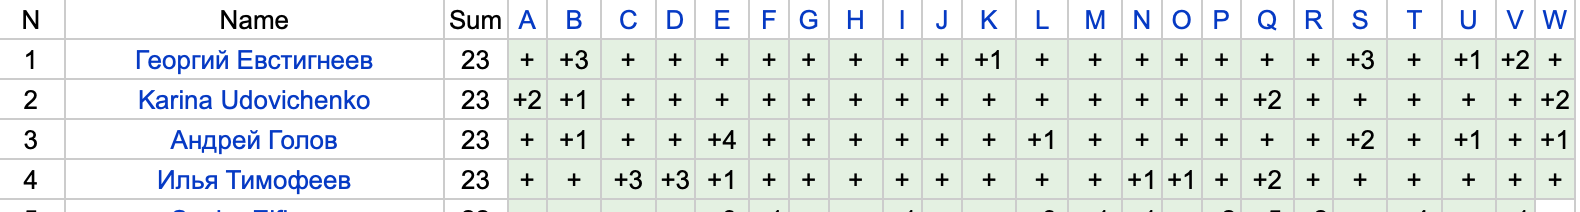
\includegraphics[width=\textwidth]{figures/monitor_acm.png}
  \caption{Монитор Информатикс для типа соревнования типа ACM}
  \label{fig:monitor_acm}
\end{figure}

\begin{figure}
  \centering
  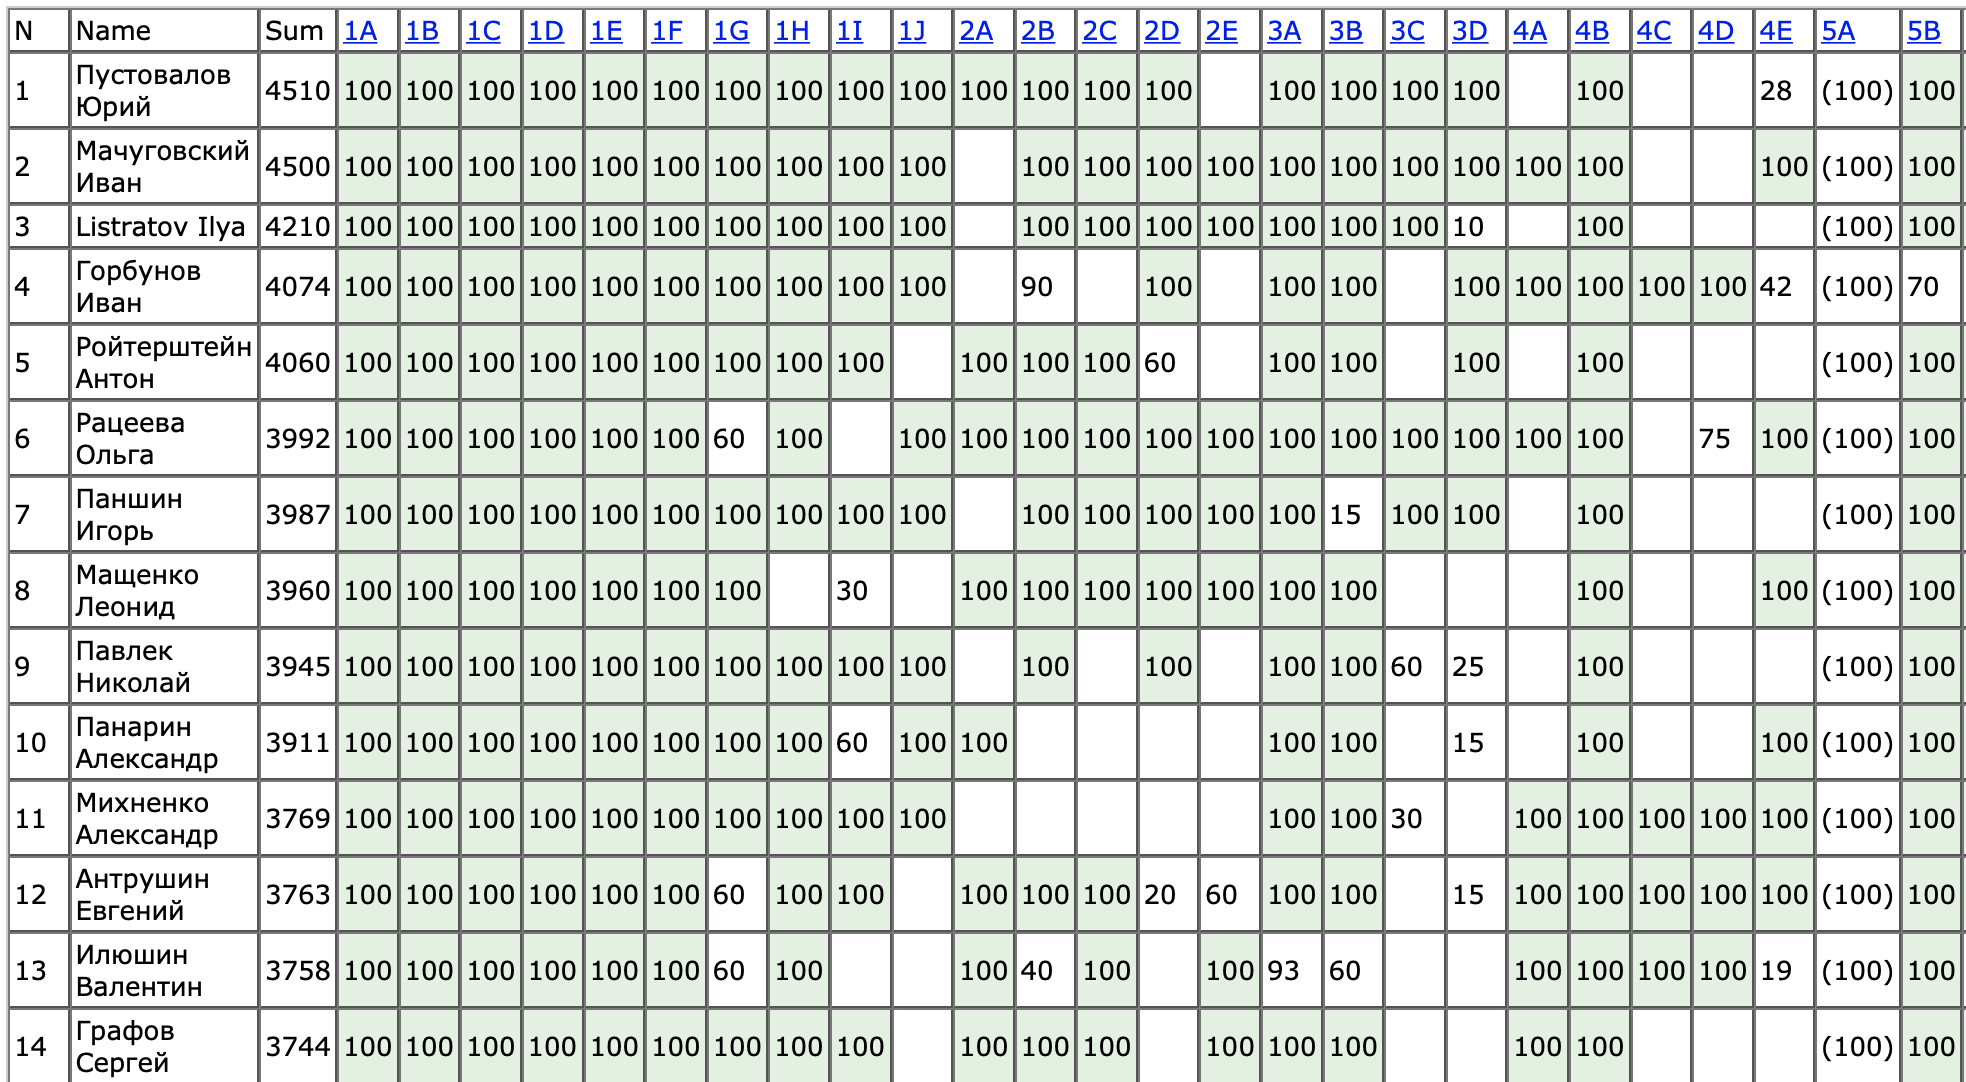
\includegraphics[width=\textwidth]{figures/monitor_ioi.png}
  \caption{Монитор Информатикс для типа соревнования типа IOI}
  \label{fig:monitor_ioi}
\end{figure}

Один сбор результатов о тестировании через новую таблицу (см. Главу \ref{lab:pynformatics_run_id}) может занимать в зависимости от общей нагрузки на БД до десятков минут, что неприемлимо.

Для того, чтобы ускорить отображение результатов прохождения учениками контестов, 
а так же уменьшить нагрузку, которую даёт сбор результатов, 
было принято решение использовать кэширующую систему\cite{cache_abstract}.

\subsection{Инвалидация кэша}

Кэширующие системы могут использовать различные приёмы для того, чтобы очищать кэш, когда он перестаёт быть валидным.
% TODO: из чего состоит кэш
Один из таких методов -- время жизни (англ. TTL -- Time To Live).
Этот метод прост в реализации, однако
при его использовании возникает проблема -- 
часть данных, отдаваемых пользователю, становится неликвидными.
Более того, чем дольше время жизни кэша, тем больше неликвидных данных получает пользователь.

Другой из методов -- очищать необходимый кэш если в системе происходят какие-либо события, изменяющие исходные данные.
Такой метод называется инвалидацией кэша.

Использовать метод, основанный только на времени жизни для результатов пользователей неверно, 
так как результаты меняются часто, и пользователям сразу важно видеть,
какое место в итоговой таблице они занимают.

Было принято использовать комбинированный метод кэширования, 
основанный как на времени жизни, так и на инвалидации кэша.

Время жизни эмпирическим путём было выбрано в одни сутки.

Код, реализующий сбор данных для монитора был реализован в системе Rmatics и представлен на листинге \ref{lst:getruns}. 
Данный код формирует данные по мониторам и возвращает их в формате JSON.

\lstinputlisting[language=Python,caption={Код, реализующий сбор данных для монитора.},label=lst:getruns]{listings/get_monitors.py}

Для инвалидации кэша результатов тестирования важно понимать, 
какие именно действия в системе приводят к изменению изначальных данных.
Эти действия -- изменения статуса посылки.
Статус посылки в БД меняется в двух случаях -- после тестирования посылки (см Рис. \ref{lab:ejudge_listener}) и при изменении статуса посылки пользователем через Web-интерфейс. 
Важно помнить, что при обновлении посылки из ejudge-listener нельзя, не используя дополнительных запросов,
получить ни идентификатор контеста, в рамках которого отправлено решение, 
ни идентификатор групп, в которых состоит пользователь, отправивший посылку.
В то же время, на этом этапе доступен идентификатор задачи и идентификатор пользователя.
Также стоит отметить, что оба действия инкапсулированы в сервис Rmatics.

Также для реализации кэша важно понимать, 
как правильно разделить кэшируемые данные.

В запросе на результаты тестирования от пользователей фигурируют следующие данные: 

\begin{itemize}
    \item Идентификатор группы пользователей.
    \item Идентификатор контеста или набор идентификаторов контестов.
    \item Ограничение по временному отрезку, в котором учитываются посылки.
\end{itemize}

Можно было бы использовать эти идентификаторы для создания ключей кэшей,
однако в таком случае каждая новая посылка любого пользователя из группы в один из контестов заставляла бы систему инвалидировать кэш,
что вело бы к постоянным повторным сборам кэшей.

Поэтому было принято разбить кэш результатов контестов на более мелкие части -- по одной на каждую задачу контеста.
В таком случае, длительность жизни каждого кэша увеличивалась,
а количество кэшей, которые нужно инвалидировать при отправке пользователем посылки -- уменьшалась.

Для того, чтобы не делать при инвалидации кэша дополнительных запросов в БД,
было решено использовать в качестве ключа кэширования не идентификатор группы,
но идентификаторы пользователей в этой группе.

\subsection{Хранение кэша}

Система, в которой хранится кэш, должна обладать следующими характеристиками:

\begin{itemize}
    \item иметь потенциальную возможность встроить инвалидацию кэша;
    \item быть удобно приспосабливаемой под задачи хранения данных типа ключ-значение;
    \item быть быстрой как для операций сохранения кэша, так и для операций выдачи данных;
    \item быть удобной в эксплуатации;
    \item желательно, чтобы система могла уметь инвалидировать значения по времени.
\end{itemize}

Рассмотрим несколько возможных вариантов для хранилища кэша.
Так как в Информатикс уже и так достаточное количество различных специфичных хранилищ, 
будем рассматривать только уже используемые на сайте системы.

Стоит сразу отбросить web-сервер nginx, так как,
хоть он и предоставляет возможность кэшировать данные,
нет никакой тривиальной возможности тривиально инвалидировать кэш после изменения статуса посылки.

Таким образом, под сравнение попадают MySQL, MongoDB и Redis. Рассмотрим так же возможность реализовать кэш на файловой системе.

\begin{center}
  \begin{longtable}{|c|c|c|c|p{0.20\textwidth}|}
    \caption{Сравнение систем для хранения кэша}
    \label{tab:cache_systems}
    \\ \hline
    Название & Ключ-значение & Скорость & Удобство & Инвалидация по времени \\
    \hline \endfirsthead
    \subcaption{Продолжение таблицы~\ref{tab:longtable}}
    \\ \hline \endhead
    \hline \subcaption{Продолжение на след. стр.}
    \endfoot
    \hline \endlastfoot
    Redis  & Да & Очень быстро & Очень удобно & Есть \\
    \hline
    MySQL  & Реализуемо & Быстро & Удобно & Нет \\
    \hline
    MongoDB  & Да & Быстро & Удобно & Нет \\
    \hline
    ФС  & Да & Медленно & Не удобно & Нет \\
    \hline
  \end{longtable}
\end{center}

По совокупности причин, приведённых выше, 
а так же по результатам сравнения в Таблице \ref{tab:cache_systems},
в качестве системы хранения кэша была выбрана СУБД Redis.

Для быстрого поиска кэша по ключу в Redis, 
было решено ограничить длину ключа, взяв MD5 хэш от аргументов запроса на выдачу данных монитора. 
MD5-хэш был создан для того, чтобы создавать компандиум (англ. message digest) для входного сообщения\cite{md5}.
Код, который используется для создания хэша от аргументов запроса представлен на листинге \ref{lst:md5}.

\lstinputlisting[language=Python,caption={Код создания хэша от аргументов запроса.},label=lst:md5]{listings/make_md5.py}

\subsection{Хранение данных для инвалидации кэша}

Для того, чтобы при обновлении статуса посылки, 
инвалидировались только нужные ключи, 
необходимо сохранить связь, между аргументами, по которым собирались данные,
в случае мониторов это идентификаторы пользователей и идентификаторы задач, 
и хэшами, эти данные хранящими.

Для этого было решено сохранять эту информацию о хэшах в СУБД MySQL.
Принимая во внимание то, что аргументы могут быть различны,
а их количество может меняться,
информацию предполагалось хранить в таблице "monitor\_cache\_meta".
Таблица должна была иметь два поля -- invalidate\_args и key.
В поле invalidate\_args должны были храниться данные об аргументах, 
с помощью которых был создан кэш, 
а в поле key должен был храниться ключ из Redis, 
по которому кэш был доступен. 

Для поля invalidate\_args ыла разработана следующая спецификация: 
аргументы, по которым собирались данные, отображались в строки, 
где сначала шло название аргумента, затем аргумент, 
и затем разделитель между аргументами.

Например, если приходили следующие аргументы, пользователь=1, пользователь=2, задача=3, а разделителем был задан символ <<|>>, то результирующей строкой было бы \textit{пользователь=1|пользователь=2|задача=3}.

В таком случае, если новая посылка пользователя 1 по задаче 3 протестировалась бы, можно было бы найти этот кэш запросом в БД,
с использованием полнотекстового поиска, например, следующим SQL-запросом:

\lstinputlisting[language=SQL,caption={Код создания хэша от аргументов запроса.},label=lst:md5]{listings/select_cache_meta.sql}

С таблицей, сохраняющей аргументы, с которыми был создан кэш,
и ключами хэшей, появилась новая проблема:
при каждой перегенерации кэша создалась запись в БД, и размер таблицы постоянно рос.
Было принято решение добавить поле "when\_expire", которое бы хранило время, когда кэш устаревал, и настроить скрипт автоматического удаления строк из БД,

Такая реализация максимально гибка; её можно использовать не только для таблиц результатов,
но и для каких-либо требующих инвалидации кэшей в будущем.

Однако, эта реализация нагружала БД, так как для инвалидации постоянно требовалось сканировать все строки "invalidate\_args"
, что доволно медленно.
Такая нагрузка была неприемлимой.
Поэтому было принято решение добавить в таблицу идентификатор задачи, "problem\_id".

Итоговая схема таблицы представлена в таблице \ref{tab:cache_meta}.

\begin{center}
  \begin{longtable}{|p{0.20\textwidth}|p{0.20\textwidth}|p{0.5\textwidth}|}
    \caption{Схема таблицы pynformatics.run}
    \label{tab:cache_meta}
    \\ \hline
    Название & Тип данных & Комментарий \\
    \hline \endfirsthead
    \subcaption{Продолжение таблицы~\ref{tab:cache_meta}}
    \\ \hline \endhead
    \hline \subcaption{Продолжение на след. стр.}
    \endfoot
    \hline \endlastfoot
    id              & INTEGER     & Идентификатор записи \\
    \hline
    key     & CAHR(128)     & Ключ в Redis \\
    \hline
    problem\_id     & INTEGER     & Идентификатор задачи \\
    \hline
    invalidate\_arg & TEXT     & Аргументы для инвалидации \\
    \hline
    when\_expire     & DATETIME     & Время, когда кэш станет невалидным \\
    \hline
  \end{longtable}
\end{center}

\subsection{Защита от гонки данных}

Существуют ситуации, в которых множество пользователей одновременно запрашивают данные результатов одного и того же соревнования.
В таких случаях происходит следующее:

\begin{enumerate}
    \item Приходит запрос на формирование данных от пользователя №1.
    \item В кэше данных ещё нет, значит, данные нужно собрать.
    \item Данные для пользователя №1 начинают собираться. 
    Как было отмечено выше, процесс сбора данных может занимать значительное время.
    \item Приходит запрос на формирование данных от пользователя №2.
    \item Данные для пользователя №1 собраны и положены в кэш.
    \item Пользователь №1 получает данные.
    \item Данные для пользователя №2 начинают собираться.
    \item Данные для пользователя №2 собраны и положены в кэш.
    Это ровно те же данные с ровно таким же ключом кэша, которые были сохранены во время обработки запроса от пользователя №1.
    \item Пользователь №2 получает данные.
\end{enumerate}

Такой порядок выполнения действий заставляет систему несколько раз собирать одни и те же данные вместо того, чтобы взять их из кэша. Более того, стоит отметить, что пользователь №2 мог получить данные гораздо позже пользователя №1, так как шаги в и ж могут выполняться долго.

Такая проблема так же может называться гонкой данных (англ. race condition)\cite{race_condition}.

Необходимо было сделать так, чтобы не смотря на то, 
что множество пользователей одновременно запрашивают данные результатов одного и того же соревнования, 
данные собирались только один раз (конечно, учитывая то, что в это время кэш может инвалидироваться).

Для этого было решено реализовать мьютекс, который блокировал бы сбор данных по определённому ключу.

Мьютекс (англ. mutex, от mutual exclusion -- <<взаимное исключение>>) -- аналог одноместного семафора, служащий для синхронизации одновременно выполняющихся потоков. 
Мьютекс отличается от семафора тем, что только владеющий им поток может его освободить, т.е. перевести в отмеченное состояние. 
В данном случае под потоками понимаются потоки выполнения запросов на сбор мониторов.

Для того, чтобы мьютекс можно было эффективно и удобно использовать в различных инстансах сервиса Rmatics, 
было решено реализовать его при помощи СУБД Redis. 
СУБД Redis имеет необходимые характеристики для того, 
чтобы эффективно реализовать мьютекс\cite{carlson2013redis}.
В качестве алгоритма был выбран алгоритм <<Redlock>>\cite{redis_lock_base}.
Этот алгоритм предоставляет возможность безопасно реализовывать блокирующие системы на кластере из СУБД Redis\cite{redis_lock_answer}.

В качестве реализации <<Redlock>> была использована библиотека <<Redlock-py>>.
Для работы системы был реализован прикладной код, реализующий логику, представленную в листинге Алгоритм \ref{alg:lock}. 

\begin{rualgorithm}[H]
 \KwData{Ключ хэша}
 \KwResult{Поток захватит мьютекс}
 инициализация\;
 Мьютекс = не захваченный Мьютекс\;
 \While{Мьютекс не захвачен}{
    Мьютекс = попытаться захватить с ключом хэша\;

  \eIf{Мьютекс не захвачен}{
  спать 0,4 секунды\;
   }{
     выйти из цикла\;
  }
 }
 \caption{Алгоритм захвата мьютекса}
 \label{alg:lock}
\end{rualgorithm}

В результате работы этого алгоритма, поток, обрабатывающий пользователя №2,
получит данные из кэша, 
и не позднее, чем через 0,4 секунды после потока (опуская время доступа к кэшу и то, что планировщик ОС может выделить время для работы потока несколько позже), обрабатывающего запрос пользователя №1.

\subsection{Выводы по подразделу}

В данной главе была рассмотрена проблема формирования данных о результатах пользователей.
Были разработаны и реализованы:

\begin{itemize}
    \item механизм кэширования данных;
    \item механизм инвалидации кэшей;
    \item механизм предотвращения гонок данных.
\end{itemize}

Иллюстрация, демонстрирующая схему работы запроса мониторов представлена на рисунке \ref{fig:cache_system}.

\begin{figure}
  \centering
  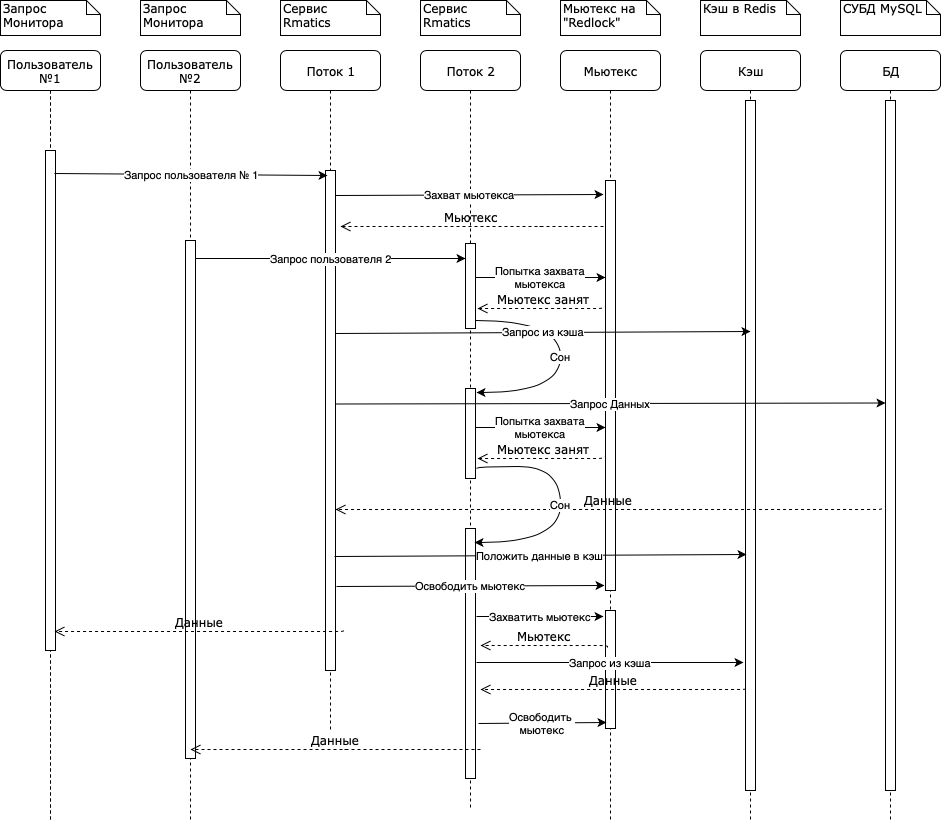
\includegraphics[width=\textwidth]{figures/cache_system.png}
  \caption{Временная диаграмма запроса мониторов двумя пользователями}
  \label{fig:cache_system}
\end{figure}
